\documentclass[UTF8]{ctexart}
%%%%%%%%%%%%%%%%%%%%%%%%%%%== 引入宏 ==%%%%%%%%%%%%%%%%%%%%%%%%%%%%%
\usepackage{cite}
\usepackage{amsmath}	% 使用数学公式
\usepackage{graphicx}	% 插入图片/PDF/EPS 等图像
\usepackage{subfigure}	% 使用子图像或者子表格
\usepackage{geometry}	% 设置页边距
\usepackage{fancyhdr}	% 设置页眉页脚
\usepackage{setspace}	% 设置行间距
\usepackage{hyperref}	% 让生成的文章目录有链接,点击时会自动跳转到该章节
\usepackage{url}
\usepackage{caption2}
\usepackage{forest}
\usepackage{float}
\usepackage{listings}
\usepackage{listings-golang}
\usepackage{color} 

\setmonofont{Monaco}

\definecolor{mygreen}{rgb}{0,0.6,0}
\definecolor{mygray}{rgb}{0.5,0.5,0.5}
\definecolor{mymauve}{rgb}{0.58,0,0.82}
\lstset{ %
  backgroundcolor=\color{white},   % choose the background color
  basicstyle=\footnotesize\ttfamily,        % size of fonts used for the code
  columns=flexible,
  breaklines=true,                 % automatic line breaking only at whitespace
  captionpos=b,                    % sets the caption-position to bottom
  tabsize=4,
  commentstyle=\color{mygreen},    % comment style
  escapeinside={\%*}{*)},          % if you want to add LaTeX within your code
  keywordstyle=\color{blue},       % keyword style
  stringstyle=\color{mymauve}\ttfamily,     % string literal style
  frame=shadowbox,
  rulesepcolor=\color{mygray},
  language=Golang,
  xleftmargin=2em,
  xrightmargin=2em, 
  aboveskip=1em
}

\def\ojoin{\setbox0=\hbox{$\bowtie$}%
  \rule[-.02ex]{.25em}{.4pt}\llap{\rule[\ht0]{.25em}{.4pt}}}
\def\leftouterjoin{\mathbin{\ojoin\mkern-5.8mu\bowtie}}
\def\rightouterjoin{\mathbin{\bowtie\mkern-5.8mu\ojoin}}
\def\fullouterjoin{\mathbin{\ojoin\mkern-5.8mu\bowtie\mkern-5.8mu\ojoin}}

%%%%%%%%%%%%%%%%%%%%%%%%%%== 设置全局环境 ==%%%%%%%%%%%%%%%%%%%%%%%%%%%%
% [geometry] 设置页边距
\geometry{top=2.6cm, bottom=2.6cm, left=2.45cm, right=2.45cm, headsep=0.4cm, foot=1.12cm}
% 设置行间距为 1.5 倍行距
\onehalfspacing
% 设置页眉页脚
\pagestyle{fancy}
%\lhead{左头标}
%\chead{\today}
%\rhead{152xxxxxxxx}
\lfoot{}
\cfoot{\thepage}
\rfoot{}
%\renewcommand{\headrulewidth}{0.4pt}
%\renewcommand{\headwidth}{\textwidth}
%\renewcommand{\footrulewidth}{0pt}

%%%%%%%%%%%%%%%%%%%%%%%%%%== 自定义命令  ==%%%%%%%%%%%%%%%%%%%%%%%%%%%%%%
% 此行使文献引用以上标形式显示
\newcommand{\supercite}[1]{\textsuperscript{\cite{#1}}}
% 此行使section中的图、表、公式编号以A-B的形式显示
\renewcommand{\thetable}{\arabic{section}-\arabic{table}}
\renewcommand{\thefigure}{\arabic{section}-\arabic{figure}}
\renewcommand{\theequation}{\arabic{section}-\arabic{equation}}
% 此行使图注、表注与编号之间的分隔符缺省,默认是冒号:
\renewcommand{\captionlabeldelim}{~}

%===================================== 标题设置  ==========================================
% \heiti \kaishu 为字体设置,ctex 会自动根据操作系统加载字体
\title{\huge{\heiti Talent-Plan Section 2}}
\author{\small{\kaishu 宋阳}\\[2pt]
\small{\kaishu 北京航空航天大学}\\[2pt]
\small{Email:}
\url{yangsoonlx@gmail.com}
}
\date{} % 去除默认日期
%\date{\today}

%===================================== 正文区域  ==========================================
\begin{document}
\maketitle
% \tableofcontents % 目录内容,注释取消掉可实现目录

\begin{flushleft}
\textbf{课程目标}:熟悉分布式计算基础 \\[8pt]
\end{flushleft}
\section{课程作业}\label{sec1}

使用Go语言,使用框架代码,用MapReduce + Shuffle的方式完成作业:从包含大量URL的数据文件中,求出现
次数最多的前10个URL和他们的出现次数,尽量利用
CPU多核特性和内存资源。
根据作业框架完成作业,详细的作业要求、框架的使用方
法和评分规则请看框架的README文件 \\

\section{课程报告}\label{sec2}

\subsection{实验结果}

下面分别展示example和自己编写的程序的执行结果,输出结果做了部分修剪

\begin{enumerate}
  \item 因为电脑性能问题,执行example会超时,所以设置了超时时间。
  \item 输出结果有些长,我就删除了一些case结果。
\end{enumerate}
\begin{lstlisting}[language={bash}]
  go test -v -run=TestExampleURLTop -timeout=20m
  === RUN   TestExampleURLTop
  Case0 PASS, dataSize=1MB, nMapFiles=5, cost=58.003091ms
  Case4 PASS, dataSize=1MB, nMapFiles=5, cost=97.798085ms
  Case0 PASS, dataSize=10MB, nMapFiles=10, cost=402.44546ms
  Case4 PASS, dataSize=10MB, nMapFiles=10, cost=1.188909096s
  Case0 PASS, dataSize=100MB, nMapFiles=20, cost=4.575127222s
  Case4 PASS, dataSize=100MB, nMapFiles=20, cost=6.447491782s
  Case0 PASS, dataSize=500MB, nMapFiles=40, cost=27.758063912s
  Case4 PASS, dataSize=500MB, nMapFiles=40, cost=24.168485049s
  Case0 PASS, dataSize=1GB, nMapFiles=60, cost=43.387110698s
  Case4 PASS, dataSize=1GB, nMapFiles=60, cost=32.157396894s
  --- PASS: TestExampleURLTop (647.35s)
  PASS
  ok  	talent	648.721s
\end{lstlisting}

\begin{lstlisting}[language={bash}]
  go test -v -run=TestURLTop -timeout=20m
  === RUN   TestURLTop
  Case0 PASS, dataSize=1MB, nMapFiles=5, cost=11.785912ms
  Case4 PASS, dataSize=1MB, nMapFiles=5, cost=41.430071ms
  Case0 PASS, dataSize=10MB, nMapFiles=10, cost=23.21466ms
  Case4 PASS, dataSize=10MB, nMapFiles=10, cost=357.336826ms
  Case0 PASS, dataSize=100MB, nMapFiles=20, cost=145.617177ms
  Case4 PASS, dataSize=100MB, nMapFiles=20, cost=3.434310151s
  Case0 PASS, dataSize=500MB, nMapFiles=40, cost=814.057602ms
  Case4 PASS, dataSize=500MB, nMapFiles=40, cost=15.216412879s
  Case0 PASS, dataSize=1GB, nMapFiles=60, cost=1.399076243s
  Case4 PASS, dataSize=1GB, nMapFiles=60, cost=29.650313254s
  --- PASS: TestURLTop (76.81s)
  PASS
  ok  	talent	78.245s
\end{lstlisting}

\subsection{实现和优化}

\textbf{任务一: 补全 mapreduce.go文件中的相应的代码。}

MRCluster.worker函数针对不同类型的任务做不同的处理,这个函数需要我们实现当任务为reduce类型的任务时需要进行的操作。
reduce任务可以分成2步:首先,reduce任务收集属于同一个关键字的所有值,这里用[]string存储一个键对应的所有值,
用$map[string] []string$来存储所有的键的信息。然后迭代map中的键值对,
交由reduceF来对每个键的值集合 进行处理并得出结果,并输出到相应的文件中。这部分的代码如下所示。
\begin{lstlisting}[language={Golang}]
  fw, bw := CreateFileAndBuf(mergeName(t.dataDir, t.jobName, t.taskNumber))
  kvMap := make(map[string] []string)
  
  for i:=0; i < t.nMap; i++ {
    rpath := reduceName(t.dataDir, t.jobName, i, t.taskNumber)
    file, err := os.Open(rpath)
    if err != nil {
      panic(err)
    }
    decoder := json.NewDecoder(file)
    for {
      var kv KeyValue
      err = decoder.Decode(&kv)
      if err != nil {
        break
      }
      if v, ok := kvMap[kv.Key]; ok{
        kvMap[kv.Key] = append(v, kv.Value)
      } else{
        kvMap[kv.Key] = []string{kv.Value}
      }
    }
    file.Close()
  }
  
  for key, value := range kvMap {
    res := t.reduceF(key, value)
    _, err := bw.Write([]byte(res))
    if err != nil {
      log.Fatal(err)
    }
  }
\end{lstlisting}

MRCluster.run函数提取来自用户提交程序的配置信息来生成相应的map和reduce任务。
我们要实现根据配置信息生成reduce任务,这部分很简单,关键在于每次任务可能分成了多个MapReduce任务,
每次MapReduce任务执行之后需要将reduce生成的结果文件名传递给notify通道,告知下一次map任务需要读取的输入文件。

\begin{lstlisting}
  rtasks := make([]*task, 0, nReduce)
  for i:=0; i < nReduce; i++ {
    t := &task{
      dataDir:    dataDir,
      jobName:    jobName,
      phase:      reducePhase,
      taskNumber: i,
      nReduce:    nReduce,
      nMap:       nMap,
      reduceF:    reduceF,
    }
    t.wg.Add(1)
    rtasks = append(rtasks, t)
    go func() { c.taskCh <- t }()
  }
  
  notifyFiles := make([]string, 0, nReduce)
  for _,t := range rtasks {
    t.wg.Wait()
    fileName := mergeName(t.dataDir, t.jobName, t.taskNumber)
    notifyFiles = append(notifyFiles, fileName)
  }
  notify <- notifyFiles
\end{lstlisting}

\textbf{任务二: 实现你自己MapF和ReduceF来计算top10。}

\textbf{example代码分析}

首先我们看一下example的实现,语言描述比较难以理解,
可以直接看图\ref{mre1}(为了简化流程,图中展示的是计算top1 url的执行过程): 
如图所示,example中的topK的计算分成了2次MapReduce来实现。

1. 第一轮,map任务为每个url生成一个键值对,每个map任务将对url做hash处理,
将url映射到不同的的reduce任务中,第一轮中的reduce任务统计每种url的出现次数,并输出结果。
具体流程如下图的round1所示,第一轮MapReduce任务执行之后,会将产生的结果文件名发送到notify管道中,交由下一轮map任务读取。
 \begin{figure}[H]
  \centering
  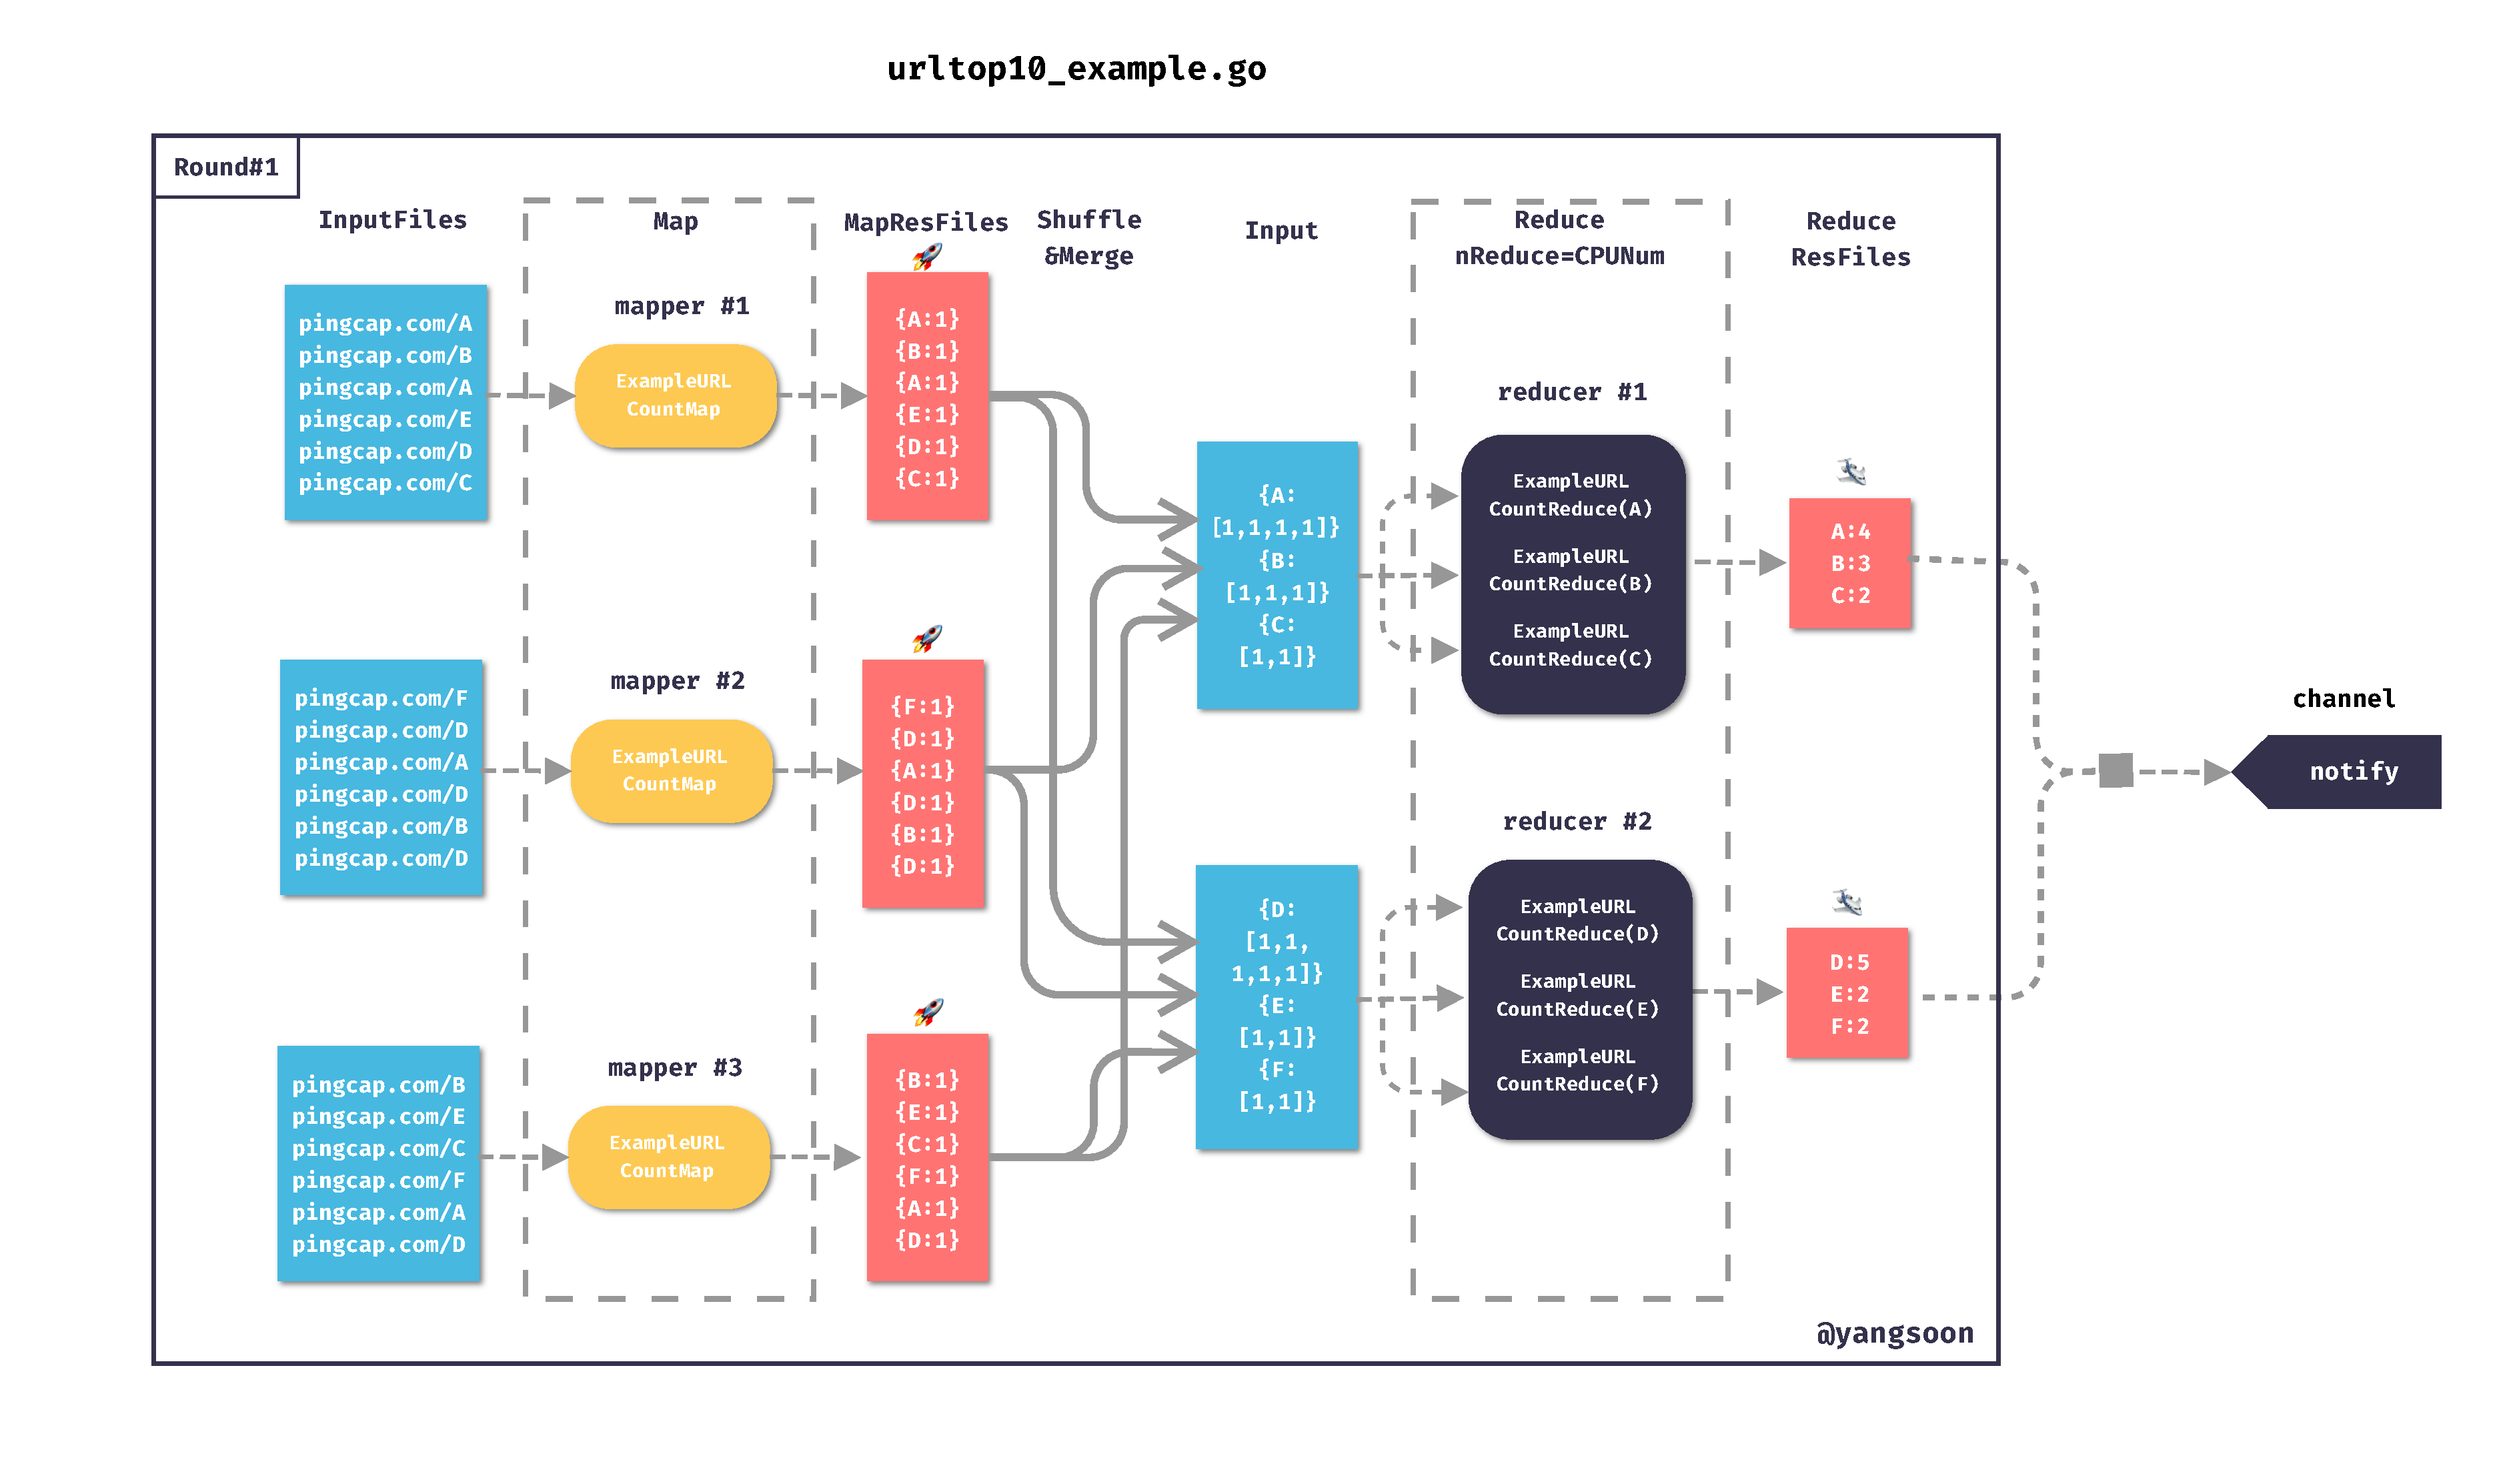
\includegraphics[width=0.9\textwidth]{fig/mr-example-1.pdf}\\
  \caption{urltop10-example-round-1}
  \label{mre1}
\end{figure}
2. 第二轮,map任务从notify管道中读取需要处理的文件,这部分map任务就是简单的将每条数据做一个键值化,
将每条url计数后的结果都分配给唯一的reduce任务,reduce任务只处理一个键值对,
其中value中存储了所有种类url的计算结果,接下来reduce任务计算出topK,
输出到唯一的一个结果文件中。具体的执行过程参考图\ref{mre2}。
\begin{figure}[H]
  \centering
  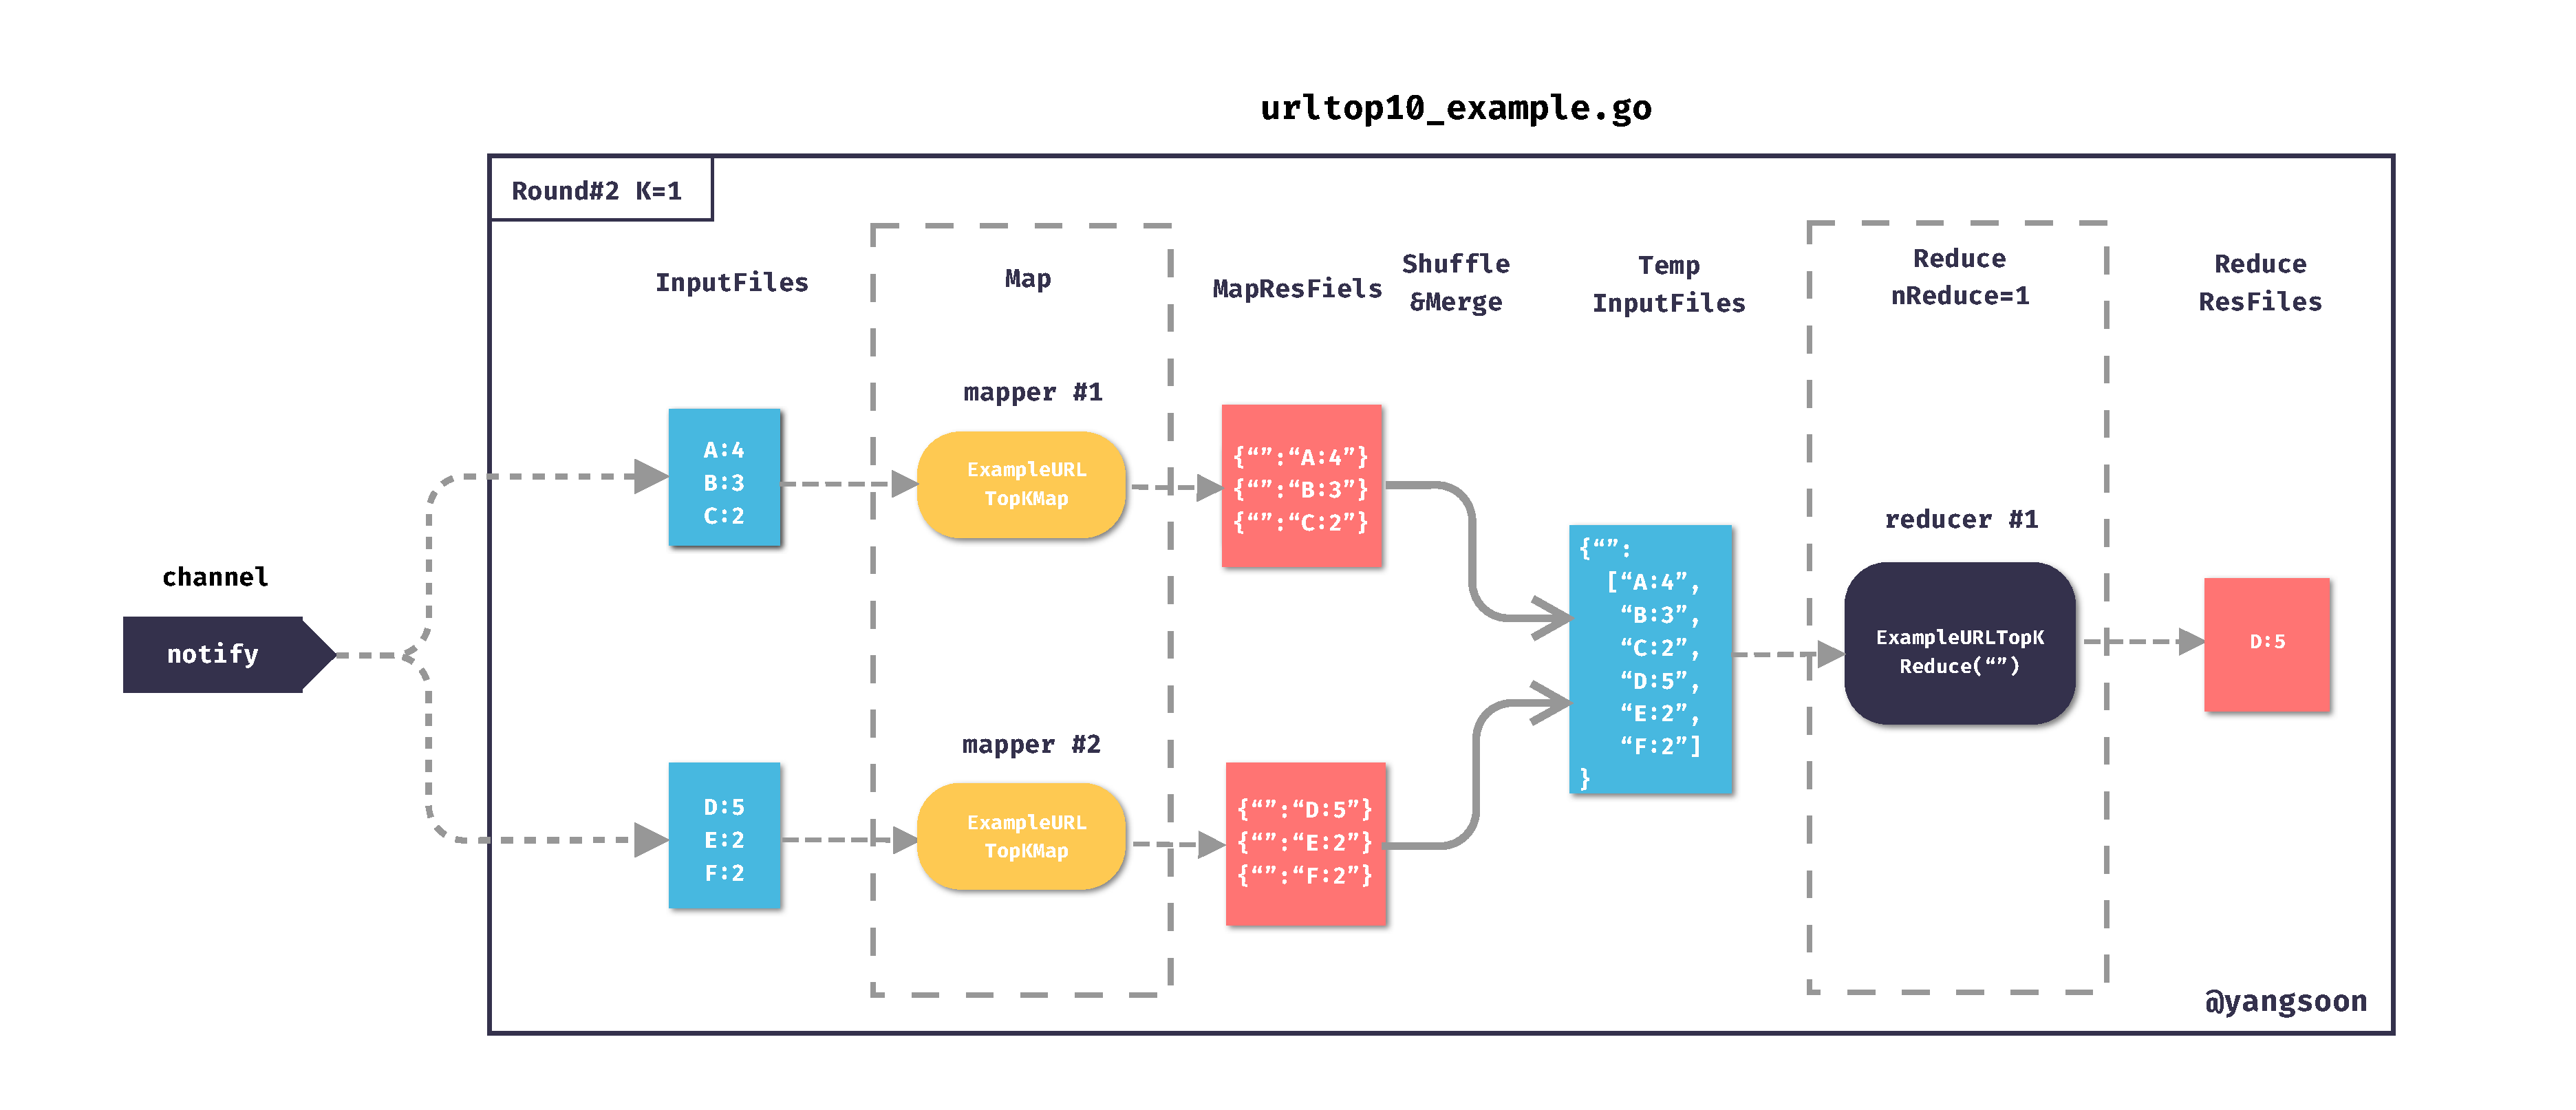
\includegraphics[width=0.7\textwidth]{fig/mr-example-2.pdf}\\
  \caption{urltop10-example-round-2}
  \label{mre2}
\end{figure}

\subsubsection{第一次优化}

当大概阅读完example的代码之后,我的第一感觉就是example代码有2处可以优化的部分:
\begin{enumerate}
  \item 首先,在第2轮的map任务就可以提前计算每个map中的top10的url,然后将结果发送给reduce任务处理,这样reduce任务的计算压力就会比较小了。
  \item 因为只需要计算出top10即可,不需要对所有的url进行排序,计算top10的算法可以使用堆进行处理,
        维护一个有10个元素的小顶堆,这样也会减少对内存的申请,减少gc时间。
\end{enumerate}

根据这样最初的想法,我实现了第一版的urltop10,和example的代码一样,
也是分成两轮,其中第一轮的代码直接复用example的代码,
第二轮的map任务使用小顶堆来计算top10,然后将结果发送给reduce任务,
reduce任务再对收集来的结果也使用小顶堆来计算top10。

但是,最终的结果不是很理想,多次执行后,时间和example相差无几,时间在630s左右。
下面是对程序的cpu性能分析结果。
\begin{lstlisting}[language=bash]
  go tool pprof cpu.prof                                                                                                      Time: Oct 4, 2019 at 5:01pm (CST)
  Duration: 10.55mins, Total samples = 24.77mins (234.68%)
  Entering interactive mode (type "help" for commands, "o" for options)
  (pprof) top
  Type: cpu
  Showing nodes accounting for 588.25s, 39.58% of 1486.06s total
  Dropped 377 nodes (cum <= 7.43s)
  Showing top 10 nodes out of 146
        flat  flat%   sum%        cum   cum%
     101.25s  6.81%  6.81%    114.77s  7.72%  encoding/json.stateInString
      76.69s  5.16% 11.97%    164.62s 11.08%  encoding/json.(*decodeState).scanWhile
      66.87s  4.50% 16.47%    189.21s 12.73%  encoding/json.checkValid
      63.91s  4.30% 20.77%     63.91s  4.30%  runtime.pthread_cond_signal
      62.79s  4.23% 25.00%    133.73s  9.00%  runtime.scanobject
      58.89s  3.96% 28.96%     79.60s  5.36%  runtime.findObject
      46.98s  3.16% 32.12%    183.71s 12.36%  runtime.mallocgc
      44.32s  2.98% 35.11%     44.33s  2.98%  encoding/json.unquoteBytes
      33.31s  2.24% 37.35%     94.69s  6.37%  runtime.gcWriteBarrier
      33.24s  2.24% 39.58%     69.77s  4.69%  runtime.mapassign_faststr
\end{lstlisting}

可以看到大部分时间都消耗在了json的解析和gc上,突然我意识到,性能瓶颈不在于排序计算,
而是在于要降低json解析的压力,那么就需要尽量减少中间文件的大小。

\subsubsection{第二次优化}

继续看example代码,还能发现几个很明显的问题,首先每一轮的map任务都在做一些很简单的事情,
只是对输入结果进行了一下简单的格式化。其次,第一轮的reduce任务每次只能在一组键值对上进行reduce操作,
但是这时候reduce任务上已经有足够的信息来计算局部的topk来对中间结果进行压缩。

根据上面的分析,我进行了第二次的优化,抛弃之前的思路,
具体的执行流程如下图所示, 问题还是通过2轮MapReduce操作进行解决。

第一轮,map任务对输入文件的url进行个数统计,计算每种url的出现次数,
得到一个url和出现次数的结果 然后在对结果格式化的时候进行一个特别的处理,
和之前的处理不同,格式化的key不再是url,而是ihash(url),就是经过hash之后的url值, 
value存储着 url: count形式的字符串,这样处理的原因是,这样处理的话
map任务中将要发送到同一个reduce work的url都会有相同的key,
这样就能保证每个reduce worker经过shuffle\&merge之后获得的输入信息是只有一个键值对的map对象,
其中包括了所有发送到该work的url统计信息;reduce任务获取到只有一个键值对的map对象后,
首先merge相同url的执行次数,然后计算局部topk,这样输出结果就只包含 K * nReduce 个信息。

\textbf{可以对比下图和上图,在标有小火箭部分的文件,
可以看到第一次中间文件的压缩结果,在标有小飞机部分的中间文件,有更加明显的数据压缩。}
\begin{figure}[H]
  \centering
  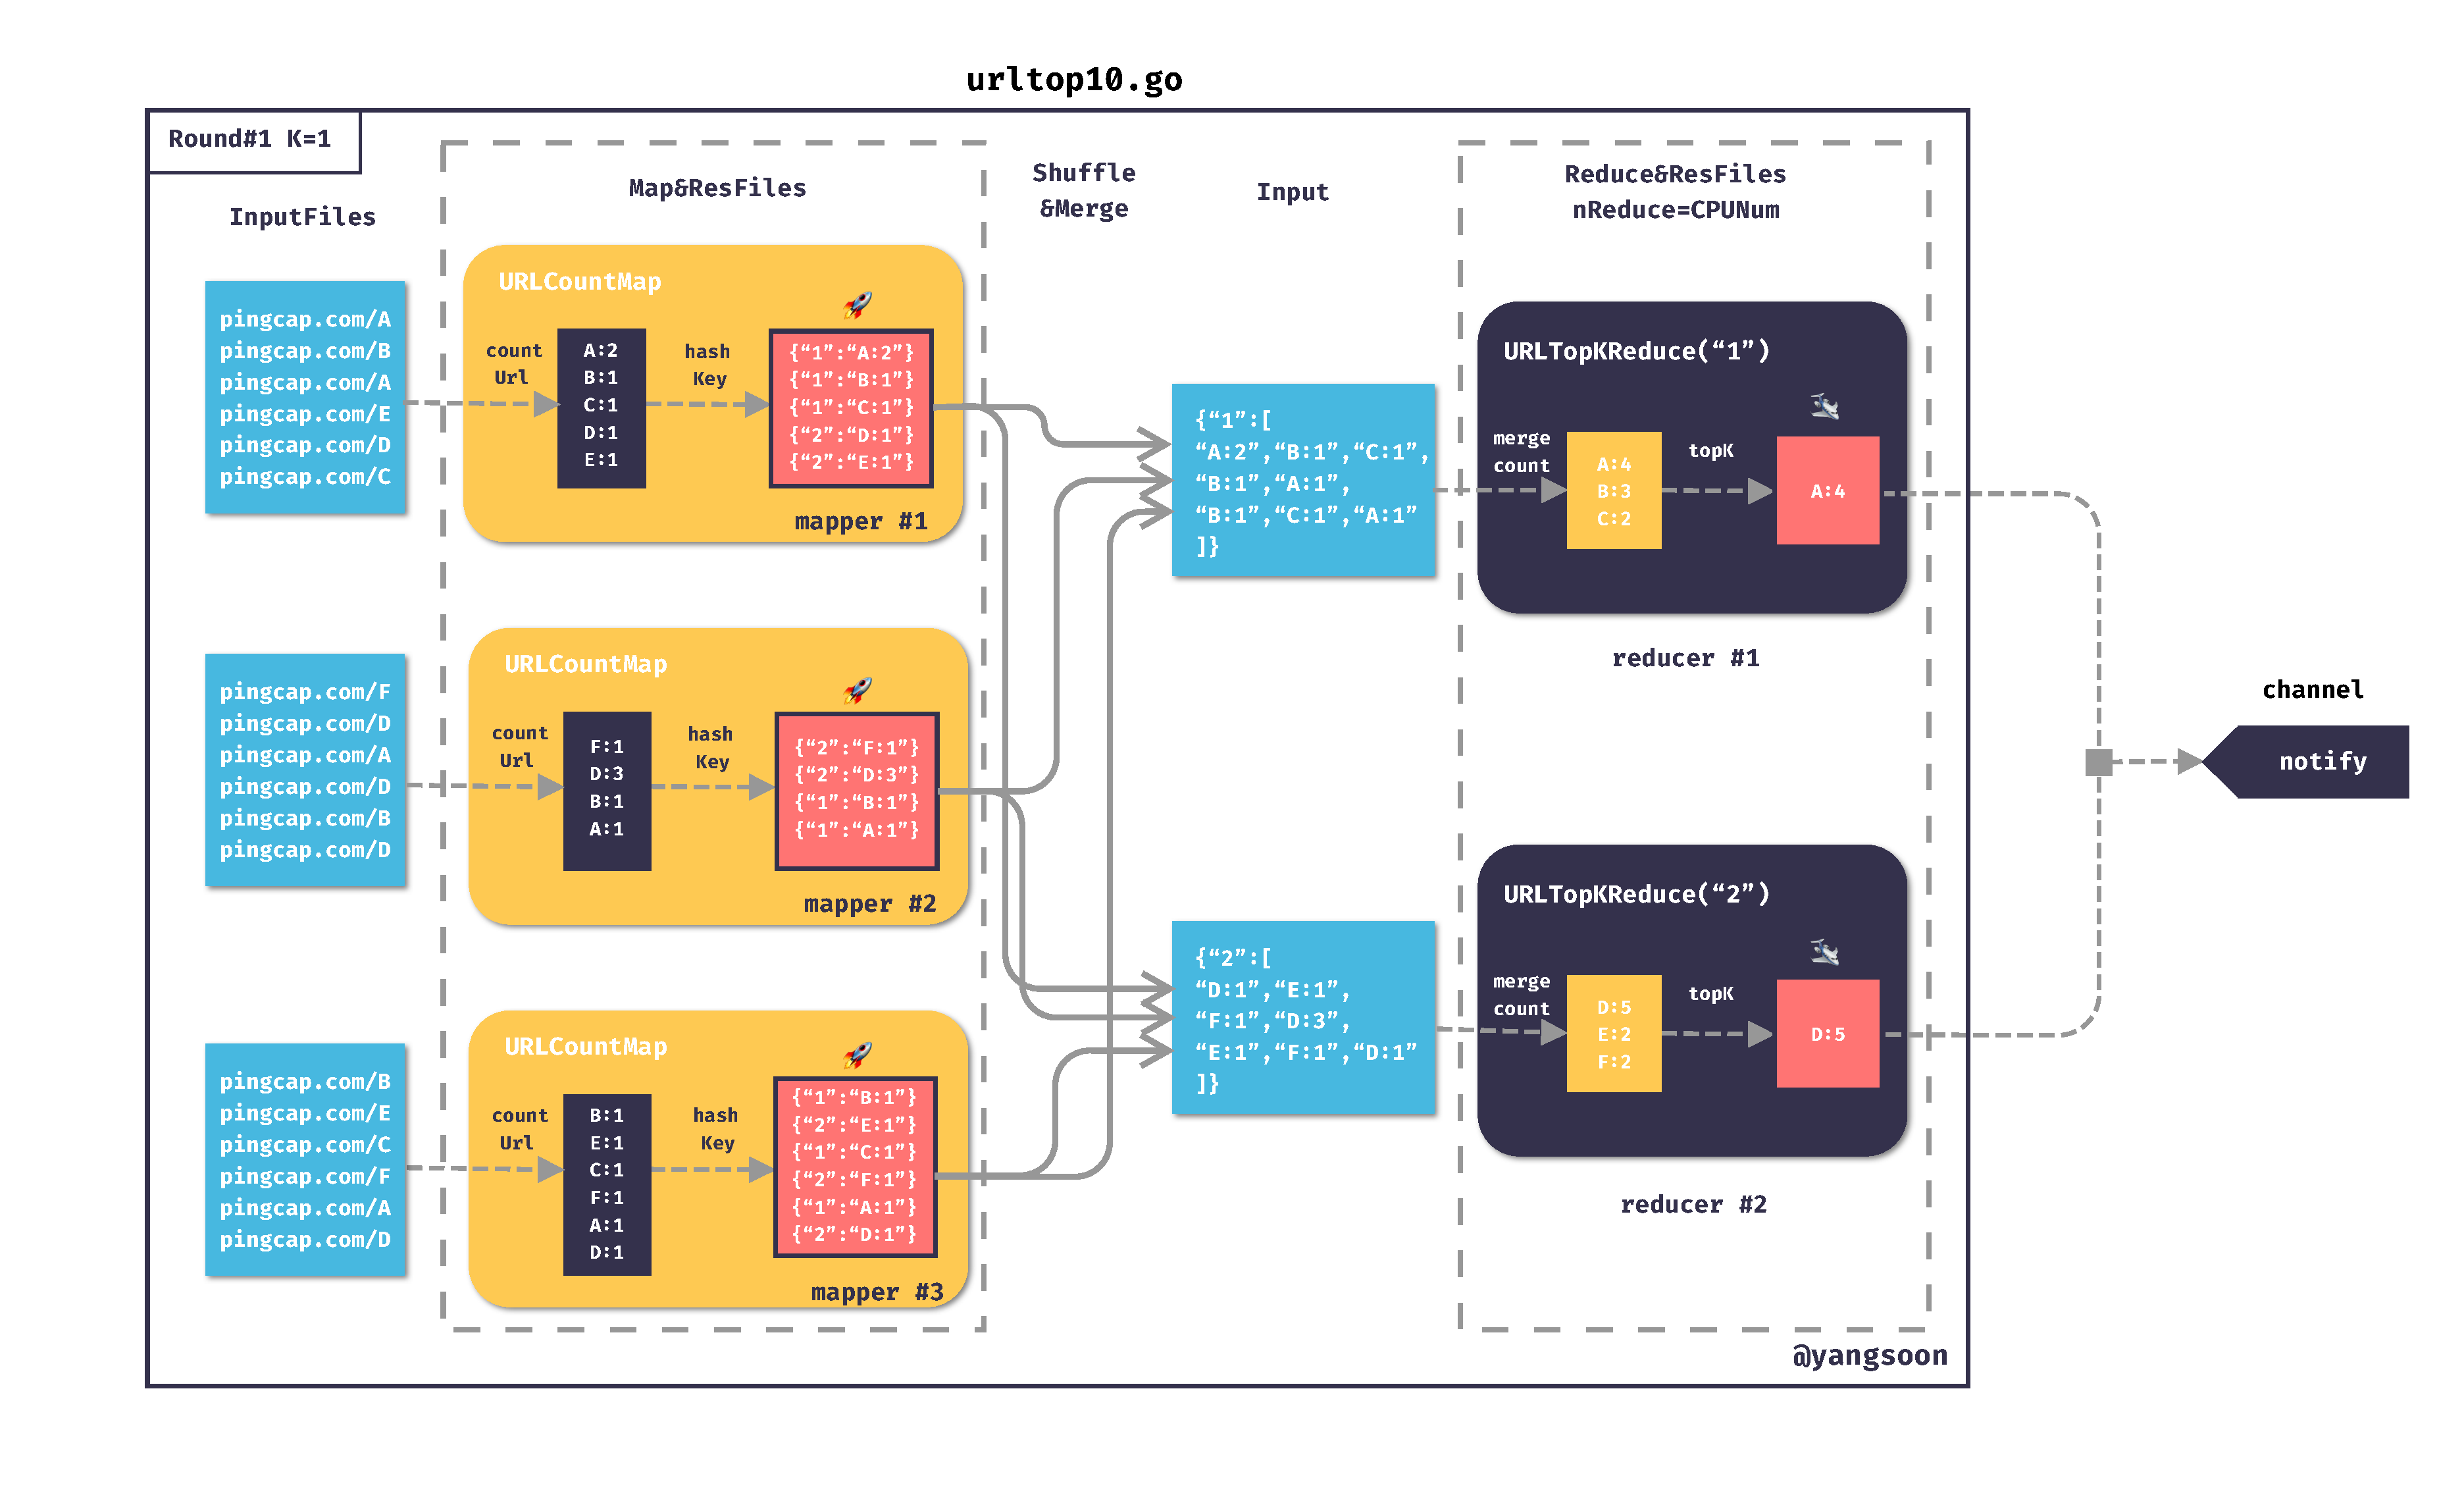
\includegraphics[width=1\textwidth]{fig/mr-1.pdf}\\
  \caption{MapReduce}
  \label{mr1}
\end{figure}
第二轮的操作和example的处理就一样了,这里就不做赘述。
\begin{figure}[H]
  \centering
  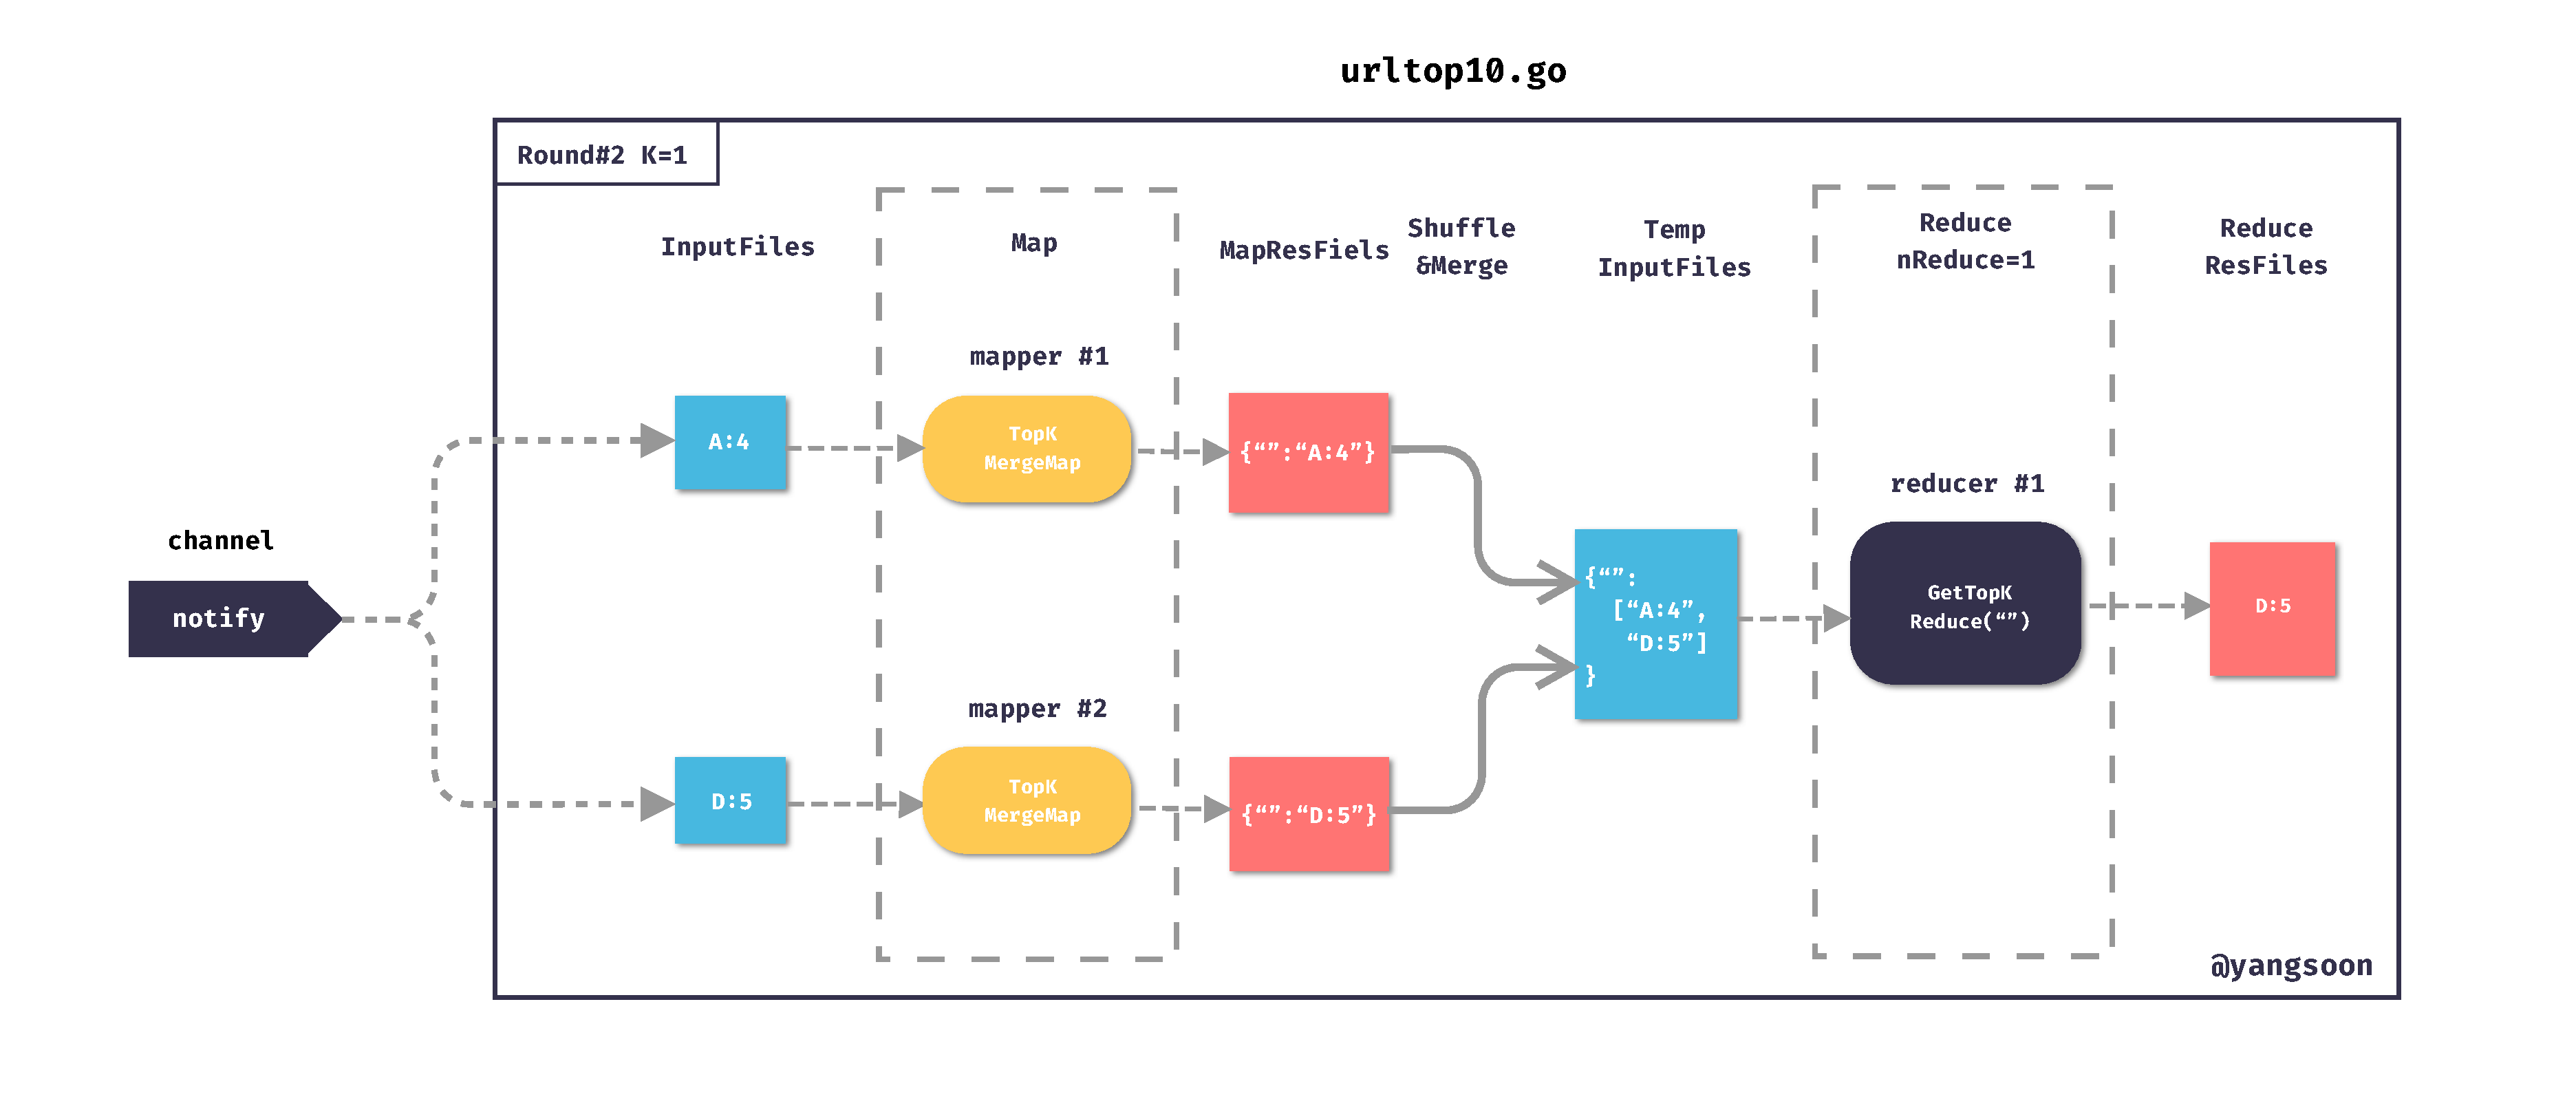
\includegraphics[width=0.9\textwidth]{fig/mr-2.pdf}\\
  \caption{MapReduce}
  \label{sec2:subsec3:fg1}
\end{figure}

之前也考虑过只用一轮MapReduce解决问题,但是思考了一下,发现并不好,
首先map worker的处理逻辑就会比较复杂,而且只能开一个reduce worker 会比较浪费cpu资源。
实际上经过一轮的压缩,第二轮能够较快的执行完。实验显示第二轮的执行时间都在1ms左右。

\textbf{部分代码}
因为主要在first round进行了优化了,所以只列出了round1的相关代码。
\begin{lstlisting}
  func URLTop10(nWorkers int) RoundsArgs {
    var args RoundsArgs
  
    args = append(args, RoundArgs{
      MapFunc:    URLCountMap,
      ReduceFunc: URLCountReduce,
      NReduce:    nWorkers,
    })
  
    args = append(args, RoundArgs{
      MapFunc:    TopKMergeMap,
      ReduceFunc: GetTopKReduce,
      NReduce:    1,
    })
  
    return args
  }
  
  func URLCountMap(filename string, contents string) []KeyValue {
    lines := strings.Split(contents, "\n")
    kv := make(map[string]int, urlKind)
    for _, l := range lines {
      if len(l) == 0 {
        continue
      }
      kv[l] += 1
    }
    kvs := make([]KeyValue, 0, len(lines))
    var buffer bytes.Buffer
    for k, v := range kv {
      buffer.WriteString(k)
      buffer.WriteString(" ")
      buffer.WriteString(strconv.Itoa(v))

      kvs = append(kvs, KeyValue{
        Key:   strconv.Itoa(ihash(k) % GetMRCluster().NWorkers()),
        Value: buffer.String(),
      })
  
      buffer.Reset()
    }
    return kvs
  }
  
  func URLCountReduce(key string, values []string) string {
  
    kv := make(map[string]int, urlKind)
  
    for _, value := range values {
      if len(value) == 0 {
        continue
      }
      tmp := strings.Split(value, " ")
      n, err := strconv.Atoi(tmp[1])
      if err != nil {
        panic(err)
      }
      kv[tmp[0]] += n
    }
  
    topk := Top10(kv)
  
    buf := new(bytes.Buffer)
    for i := 0; i < len(topk); i++ {
      fmt.Fprintf(buf, "%s %d\n", topk[i].url, topk[i].cnt)
    }
    return buf.String()
  }  
\end{lstlisting}

\subsection{性能分析}

\textbf{CPU}
cpu性能分析的结果\ref{cpu}上来看,syscall.syscall调用耗费了大量的时间,从火焰图上能够看出是因为进行json解析文件产生的大量IO耗时。
除了syscall.syscall之外几个函数都是和gc相关的函数调用。$runtime.mapassign\_faststr$执行时间过多,是因为在URLCountMap函数中计算每种
URL的个数所以会频繁的查找map,更新map。strings.genSplit是由于需要对传递给URLCountMap的数据根据换行符切片导致的大量时间消耗。

\begin{lstlisting}[language=bash]
  go tool pprof cpu.prof                                                                            
  Type: cpu
  Time: Jan 4, 2020 at 9:31pm (CST)
  Duration: 1.28mins, Total samples = 3.89mins (303.12%)
  Entering interactive mode (type "help" for commands, "o" for options)
  (pprof) top
  Showing nodes accounting for 159.20s, 68.29% of 233.14s total
  Dropped 295 nodes (cum <= 1.17s)
  Showing top 10 nodes out of 133
        flat  flat%   sum%        cum   cum%
      93.42s 40.07% 40.07%     93.53s 40.12%  syscall.syscall
      12.22s  5.24% 45.31%     30.66s 13.15%  runtime.mapassign_faststr
       8.94s  3.83% 49.15%     18.70s  8.02%  runtime.scanobject
       7.88s  3.38% 52.53%      7.88s  3.38%  runtime.memmove
       7.07s  3.03% 55.56%      7.07s  3.03%  runtime.madvise
       6.98s  2.99% 58.55%      9.04s  3.88%  runtime.findObject
       6.95s  2.98% 61.53%      6.95s  2.98%  aeshashbody
       5.88s  2.52% 64.06%     23.07s  9.90%  strings.genSplit
       4.94s  2.12% 66.17%      4.94s  2.12%  memeqbody
       4.92s  2.11% 68.29%      4.92s  2.11%  runtime.memclrNoHeapPointers
\end{lstlisting}

\begin{figure}[H]
  \caption{CPU火焰图}
  \label{cpu}
  \centering
  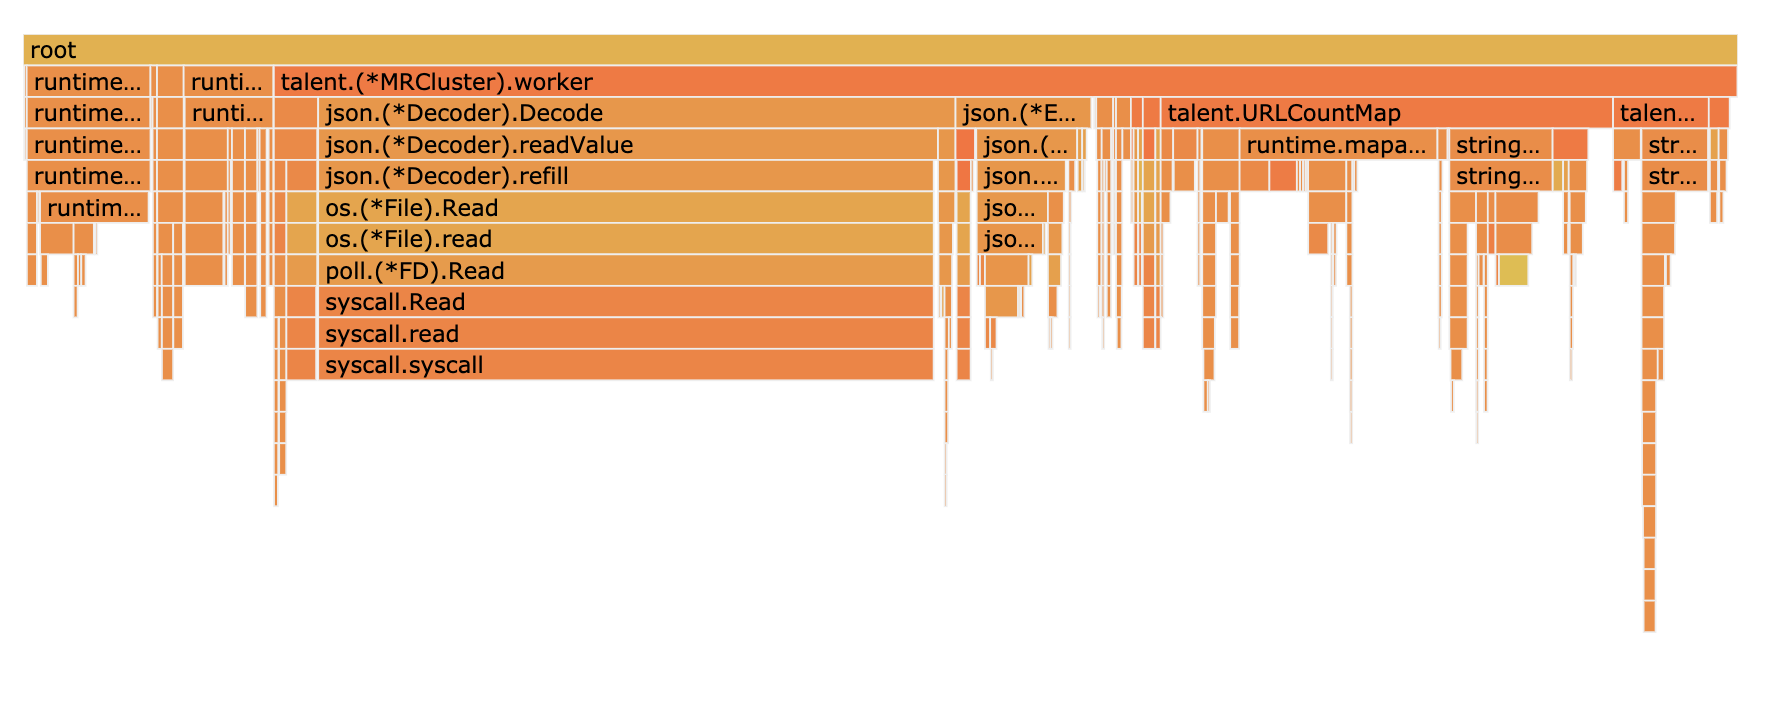
\includegraphics[width=1\textwidth]{fig/cpu.png}\\
\end{figure}

\subsubsection{JSON解析分析}
因为官方自带的json解析器性能确实有待提升,所以就将官方的json解析器替换成
json-iterator,优化后的执行结果上来看确实有提升,但是和修改之前相比也就快了几秒的时间。
\label{op-json}
\begin{lstlisting}[language=bash]
  --- PASS: TestURLTop (76.81s)
  PASS
  ok  	talent	78.245s
  
  --- PASS: TestURLTop (72.64s)
  PASS
  ok  	talent	74.104s
\end{lstlisting}

\subsubsection{MEM分析}

从分析结果上来看,worker和URLCountMap有较多的内存分配,其中URLCountMap是用户编写的代码,通过list命令查看URLCountMap函数发现是因为对map更新的
时候map扩容导致的大量内存分配,因为map大小和数据中URL的种类有关,我就用一个URLKind的变量来表示初始化map的大小。这个变量和数据相关,就先这样处理,
然后strings.Split函数导致的。通过图\ref{cpu-graph}能明显看到这几个函数执行时间耗费了较多的时间。最后还有一部分是因为自己实现代码的时候写出了bug,
也是通过list查看发现的,因为太蠢了就不列出来了。

\begin{lstlisting}[language=bash]
  go tool pprof mem.prof
  Type: alloc_space
  Time: Jan 4, 2020 at 9:32pm (CST)
  Entering interactive mode (type "help" for commands, "o" for options)
  (pprof) top
  Showing nodes accounting for 100GB, 98.49% of 101.54GB total
  Dropped 50 nodes (cum <= 0.51GB)
  Showing top 10 nodes out of 25
        flat  flat%   sum%        cum   cum%
     25.67GB 25.28% 25.28%    25.67GB 25.28%  github.com/json-iterator/go.NewStream
     22.61GB 22.27% 47.55%   101.53GB   100%  talent.(*MRCluster).worker
     17.70GB 17.43% 64.98%    17.70GB 17.43%  bytes.makeSlice
     10.87GB 10.71% 75.69%    23.80GB 23.44%  talent.URLCountMap
     10.62GB 10.46% 86.15%    10.62GB 10.46%  strings.genSplit
      6.23GB  6.14% 92.29%     6.23GB  6.14%  bufio.NewWriterSize
      1.96GB  1.93% 94.22%     2.41GB  2.38%  github.com/json-iterator/go.(*Iterator).ReadString
      1.88GB  1.85% 96.07%     2.56GB  2.52%  talent.ihash
      1.78GB  1.75% 97.82%     1.78GB  1.75%  bytes.(*Buffer).String
      0.68GB  0.67% 98.49%     0.68GB  0.67%  hash/fnv.New32a
\end{lstlisting}

\begin{figure}[H]
  \centering
  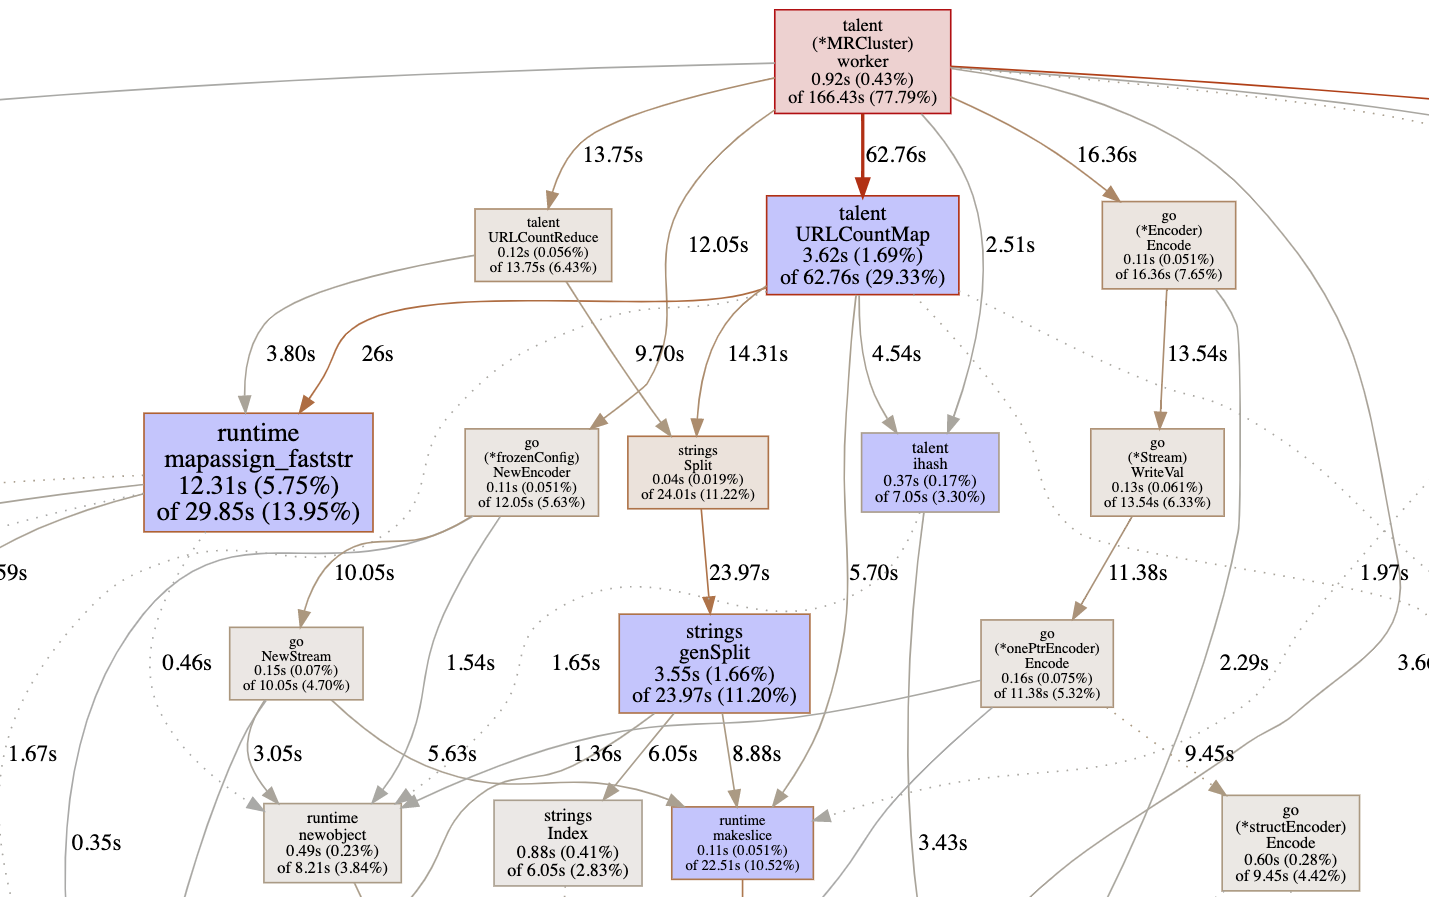
\includegraphics[width=0.8\textwidth]{fig/cpu-graph.png}\\
  \caption{cpu-graph}
  \label{cpu-graph}
\end{figure}
go.NewStream函数内存分配排到了第一,我们用list命令看一下具体的内存分配情况。
从第106行可以看到,因为每次遍历kvs的时候都会初始化一遍Encoder,实际上Encoder初始化nReduce次就足够了,
这里可以修改一下,提前初始化Encoder。因为这部分是框架上的代码,修改之后我会注释掉。
\begin{lstlisting}[language=bash]
  Type: alloc_space
  Time: Jan 5, 2020 at 1:33pm (CST)
  Entering interactive mode (type "help" for commands, "o" for options)
  (pprof) list worker
  Total: 101.54GB
  ROUTINE ======================== talent.(*MRCluster).worker in /Users/yangs/Projects/talent-plan/tidb/mapreduce/mapreduce.go
     22.61GB   101.53GB (flat, cum)   100% of Total
           .          .     88:	defer c.wg.Done()
           .          .     ........................
           .          .     98:				fs := make([]*os.File, t.nReduce)
           .          .     99:				bs := make([]*bufio.Writer, t.nReduce)
           .          .    100:				for i := range fs {
           .   512.03kB    101:					rpath := reduceName(t.dataDir, t.jobName, t.taskNumber, i)
           .     5.97GB    102:					fs[i], bs[i] = CreateFileAndBuf(rpath)
           .          .    103:				}
     17.69GB    41.49GB    104:				results := t.mapF(t.mapFile, string(content))
           .          .    105:				for _, kv := range results {
           .    26.64GB    106:					enc := json.NewEncoder(bs[ihash(kv.Key)%t.nReduce])
           .      350MB    107:					if err := enc.Encode(&kv); err != nil {
           .          .    108:						log.Fatalln(err)
           .          .    109:					}
           .          .    110:				}
\end{lstlisting}

经过优化后,我们可以看到go.NewStream已经不在top10了,而且URLCountMap的内存分配也降低了很多。
\begin{lstlisting}[language=bash]
  go tool pprof mem.prof
  Type: alloc_space
  Time: Jan 5, 2020 at 4:42pm (CST)
  Entering interactive mode (type "help" for commands, "o" for options)
  (pprof) top
  Showing nodes accounting for 73.17GB, 98.11% of 74.58GB total
  Dropped 56 nodes (cum <= 0.37GB)
  Showing top 10 nodes out of 32
        flat  flat%   sum%        cum   cum%
     22.66GB 30.38% 30.38%    74.57GB   100%  talent.(*MRCluster).worker
     17.69GB 23.72% 54.10%    17.69GB 23.72%  bytes.makeSlice
     10.60GB 14.21% 68.31%    10.60GB 14.21%  strings.genSplit
      6.25GB  8.38% 76.69%     6.25GB  8.38%  bufio.NewWriterSize
      5.06GB  6.79% 83.48%    18.09GB 24.26%  talent.URLCountMap
      4.48GB  6.01% 89.49%     4.48GB  6.01%  github.com/json-iterator/go.(*Stream).WriteStringWithHTMLEscaped
      2.12GB  2.84% 92.33%     2.61GB  3.50%  talent.ihash
      1.97GB  2.64% 94.97%     2.40GB  3.21%  github.com/json-iterator/go.(*Iterator).ReadString
      1.85GB  2.48% 97.45%     1.85GB  2.48%  bytes.(*Buffer).String
      0.49GB  0.66% 98.11%     0.49GB  0.66%  hash/fnv.New32a
\end{lstlisting}

和初始版本相比执行时间快了几秒。
\begin{lstlisting}[language=bash]
  --- PASS: TestURLTop (76.81s)
  PASS
  ok  	talent	78.245s
  --- PASS: TestURLTop (68.05s)
  PASS
  ok  	talent	68.792s
\end{lstlisting}

\end{document}
